\documentclass[12pt, titlepage]{article}

\usepackage{fullpage}
\usepackage[round]{natbib}
\usepackage{multirow}
\usepackage{booktabs}
\usepackage{tabularx}
\usepackage{graphicx}
\usepackage{longtable}
\usepackage{float}
\usepackage{hyperref}
\hypersetup{
	colorlinks,
	citecolor=blue,
	filecolor=black,
	linkcolor=red,
	urlcolor=blue
}

%% Comments

\usepackage{color}

\newif\ifcomments\commentstrue %displays comments
%\newif\ifcomments\commentsfalse %so that comments do not display

\ifcomments
\newcommand{\authornote}[3]{\textcolor{#1}{[#3 ---#2]}}
\newcommand{\todo}[1]{\textcolor{red}{[TODO: #1]}}
\else
\newcommand{\authornote}[3]{}
\newcommand{\todo}[1]{}
\fi

\newcommand{\wss}[1]{\authornote{blue}{SS}{#1}} 
\newcommand{\plt}[1]{\authornote{magenta}{TPLT}{#1}} %For explanation of the template
\newcommand{\an}[1]{\authornote{cyan}{Author}{#1}}

%% Common Parts

\newcommand{\progname}{ProgName} % PUT YOUR PROGRAM NAME HERE
\newcommand{\authname}{Team \#, Team Name
\\ Student 1 name and macid
\\ Student 2 name and macid
\\ Student 3 name and macid
\\ Student 4 name and macid} % AUTHOR NAMES                  

\usepackage{hyperref}
    \hypersetup{colorlinks=true, linkcolor=blue, citecolor=blue, filecolor=blue,
                urlcolor=blue, unicode=false}
    \urlstyle{same}
                                


\newcounter{acnum}
\newcommand{\actheacnum}{AC\theacnum}
\newcommand{\acref}[1]{AC\ref{#1}}

\newcounter{ucnum}
\newcommand{\uctheucnum}{UC\theucnum}
\newcommand{\uref}[1]{UC\ref{#1}}

\newcounter{mnum}
\newcommand{\mthemnum}{M\themnum}
\newcommand{\mref}[1]{M\ref{#1}}

\begin{document}
	
	\title{System Design for \progname{}} 
	\author{\authname}
	\date{\today}
	
	\maketitle
	
	\pagenumbering{roman}
	
	\section{Revision History}
	
	\begin{tabularx}{\textwidth}{p{3cm}p{2cm}X}
		\toprule {\bf Date} & {\bf Version} & {\bf Notes}\\
		\midrule
		January 17, 2023 & 1.0 & Initial document created\\
		January 18, 2023 & 1.1 & UI images added\\
		January 18, 2023 & 1.2 & Remaining document completed\\
		April 5 & 1.5 & Final document changes \\
		\bottomrule
	\end{tabularx}
	
	\newpage
	
	\section{Reference Material}
	
	This section records information for easy reference.
	
	\subsection{Abbreviations and Acronyms}
	
	\renewcommand{\arraystretch}{1.2}
	\begin{table}[H]
		\small
		\centering
		\begin{tabular}{l p{15cm}} 
			\toprule		
			\textbf{symbol} & \textbf{description}\\
			\midrule
			API & Application Programming Interface refers to a software with a distinct function\\
			CSS & Cascading Style Sheets, a language used to design the style of a website page\\
			GitHub & Internet hosting service for software development and version control using Git\\
			HTTP & Hypertext Transfer Protocol, a protocol used to communicate over the internet\\
			REST & Representational state transfer is a software architectural style that describes the architecture of the Web\\
			SRS & Software Requirement Specification\\
			TCP & Transmission Control Protocol, a protocol used to communicate over the internet\\
			UI & User Interface, usually refers to components of a system that can be viewed and interacted with\\
			\bottomrule
		\end{tabular}
	\end{table}
	
	\newpage
	
	\tableofcontents
	
	\newpage
	
	\listoftables
	
	\listoffigures
	
	\newpage
	
	\pagenumbering{arabic}
	
	\section{Introduction}
	UnderTree is a collaborative LaTeX document editor that supports GitHub version control for projects. The aim of this software, as discussed in the Problem Statement, is to provide the ability for multiple people to edit LaTeX documents concurrently while viewing real time changes. The stakeholders involved, as discussed in the SRS, include the developers, enterprises, people interested in LaTeX documentation with version control, and researchers.
	
	This document will discuss system design decisions related to UnderTree.
	
	\section{Purpose}
	The purpose of this document is to outline the design decisions for the project as outlined in the MG and MIS, and map them to the requirements. The document defines the scope of the system, then gives a project overview which outlines the normal behaviour of the system, any undesired event handling, a component diagram and a mapping of design decisions to requirements (as outlined in the SRS). Then it will discuss any system variables and a thorough walkthrough of the user interface design will be provided. Finally, communication protocols and a timeline of implementation will be discussed.
	
	\section{Scope}
	
	Reference the context diagram in the \href{https://github.com/RutheniumVI/UnderTree/blob/main/docs/SRS/SRS.pdf}{SRS}
	
	\section{Project Overview}
	
	\subsection{Normal Behaviour}
	
	This application is to be user for collaborative LaTeX editing. Users will also be able to login to the application using their GitHub account. The application also supports version control for the LaTeX projects. The users are able to import or create new project to GitHub. They can then edit the LaTeX documents in a project concurrently while viewing real time changes from other collaborators of the project. After editing files, the users are also able to commit their changes to GitHub. 
	
	\subsection{Undesired Event Handling}
	
	When an undesired event happens, the system is designed to log the error and be able to continue operation like usual. In case there is an error during an API call to the server, the system will pass on the error to the caller as debug information. Events are also logged to a local file which can be viewed at a later time. In case of an authentication error, all further action is halted for the task to prevent security risks.
	
	\subsection{System Context Diagram}
	
	\begin{figure}[H]
		\centering
		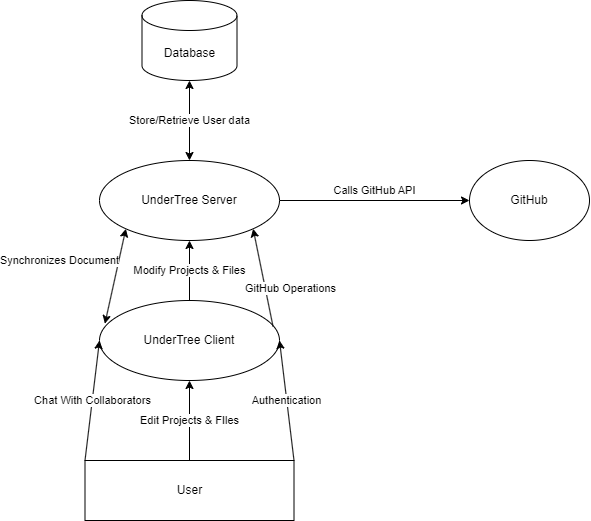
\includegraphics[scale=0.7]{system_context.png}
		\caption{Context Diagram of UnderTree}
	\end{figure}
	
	% \subsection{Component Diagram}
	
	
	
	% \subsection{Connection Between Requirements and Design} \label{SecConnection}
	
	% \wss{The intention of this section is to document decisions that are made
		%   ``between'' the requirements and the design.  To satisfy some requirements,
		%   design decisions need to be made.  Rather than make these decisions implicit,
		%   they are explicitly recorded here.  For instance, if a program has security
		%   requirements, a specific design decision may be made to satisfy those
		%   requirements with a password.}
	
	\section{System Variables}
	
	N/A
	
	\section{User Interfaces}
	
	The following screenshots show the user interface design for this project. This User Interface is built focusing only on desktop design, we do not care much about mobile responsiveness since this web application is built to be used on a desktop. However these designs should still be responsive for various screensizes:
	
	\begin{figure}[H]
		\centering
		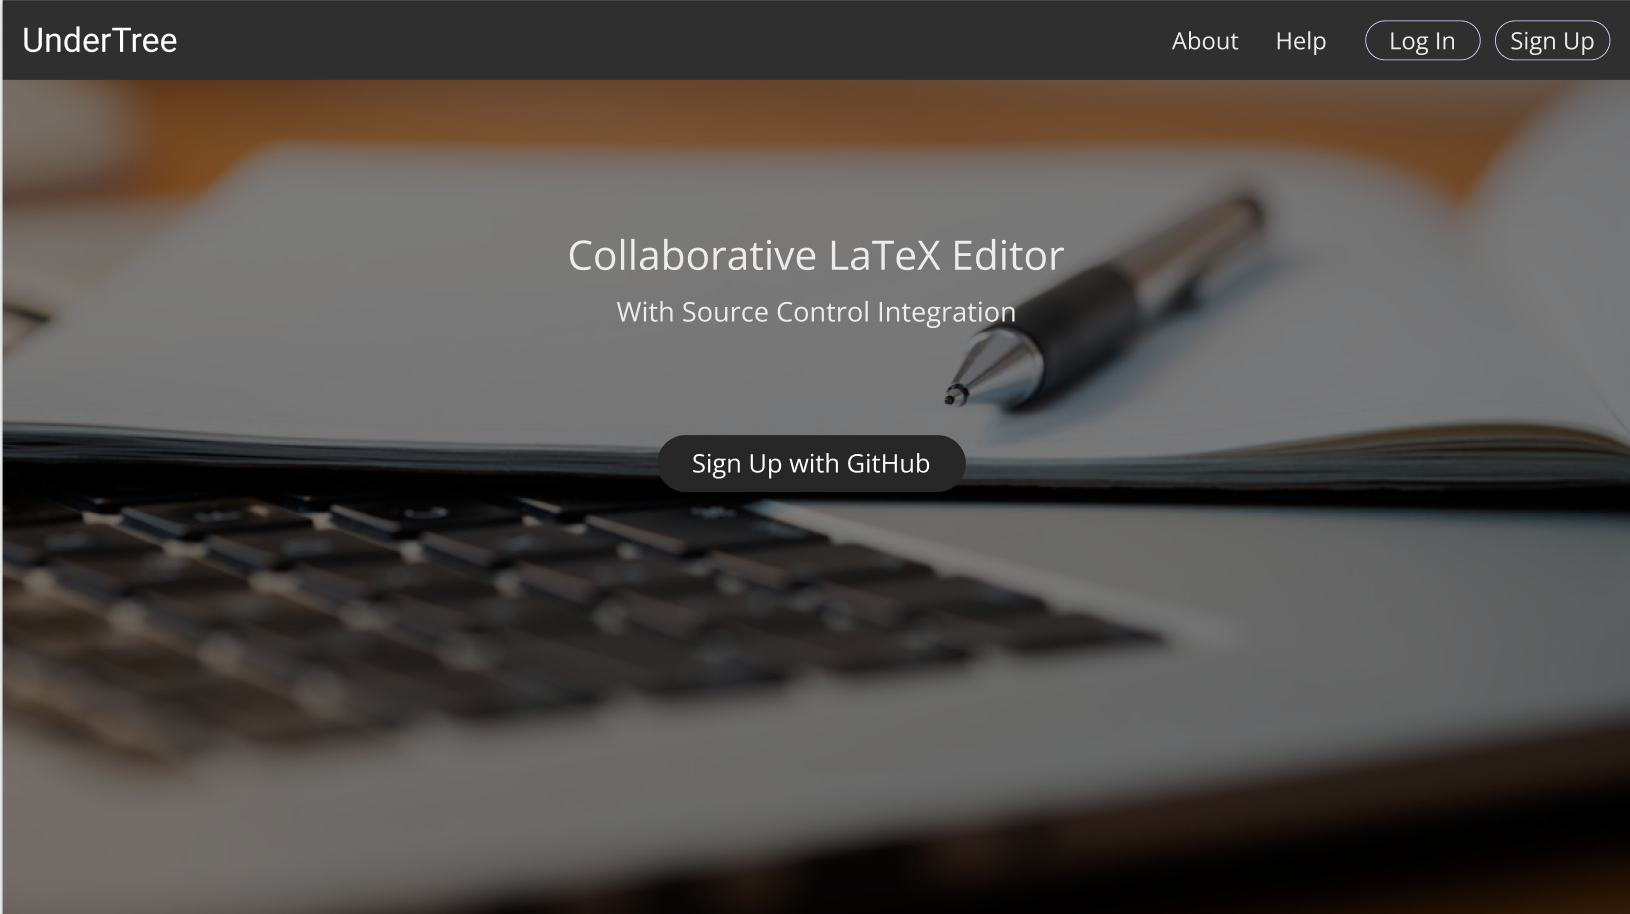
\includegraphics[width=\linewidth]{homePage.png}
		\caption{User interface of the home page}
	\end{figure}
	
	\begin{figure}[H]
		\centering
		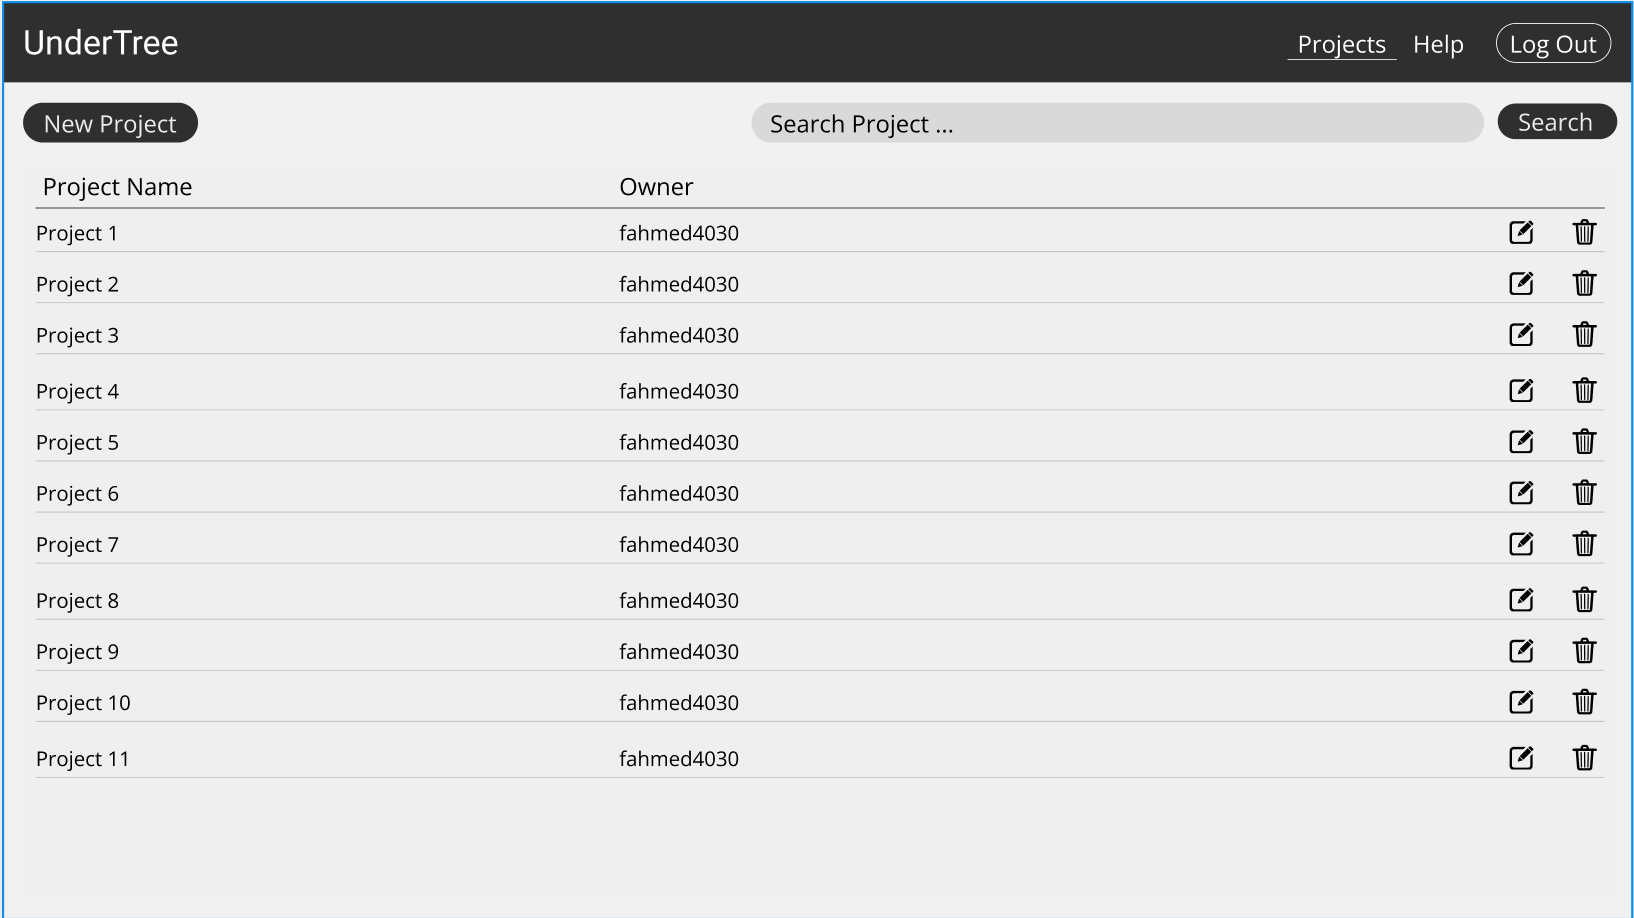
\includegraphics[width=\linewidth]{projectsPage.png}
		\caption{User interface of the projects page}
	\end{figure}
	
	\begin{figure}[H]
		\centering
		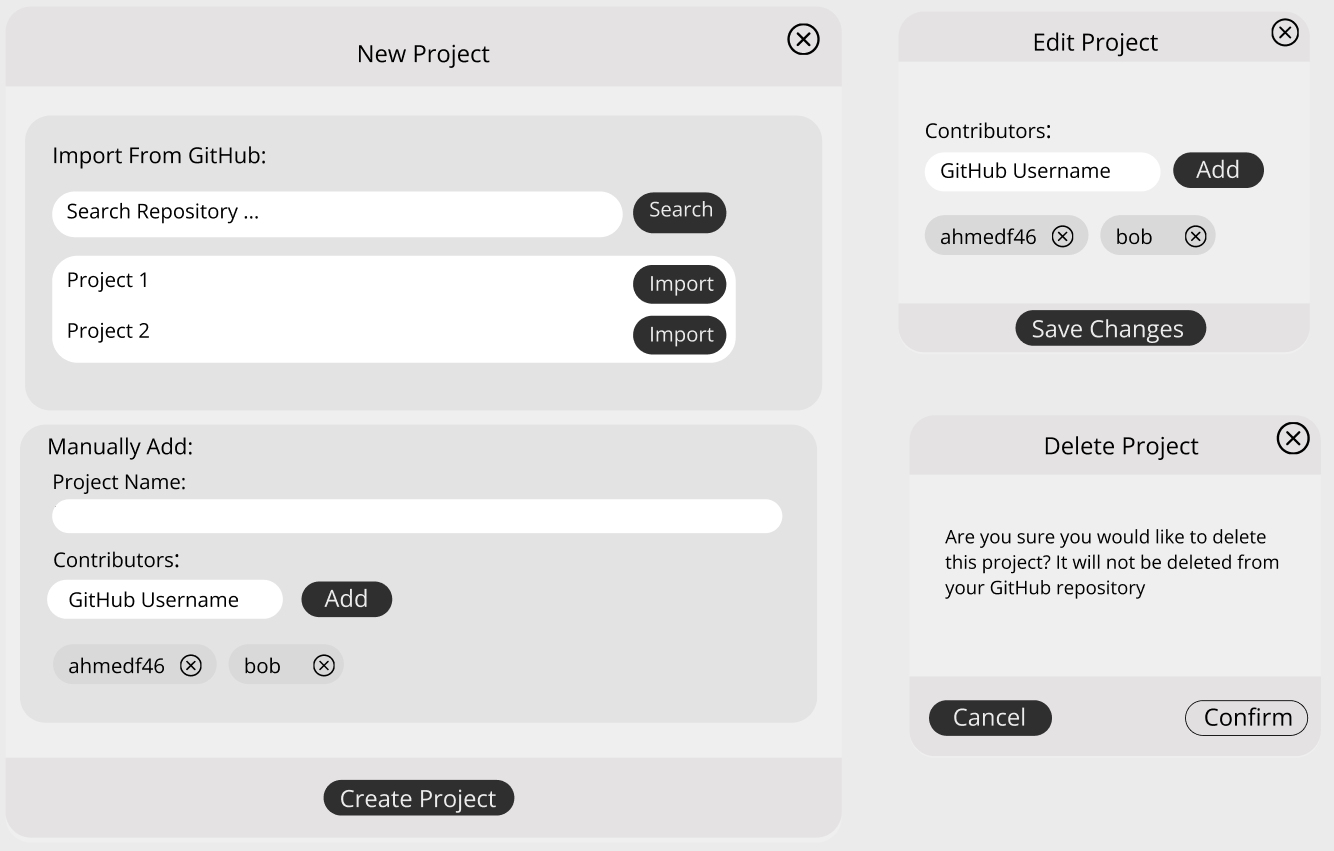
\includegraphics[width=\linewidth]{projectModals.png}
		\caption{User interface of the project modals/popups}
	\end{figure}
	
	\begin{figure}[H]
		\centering
		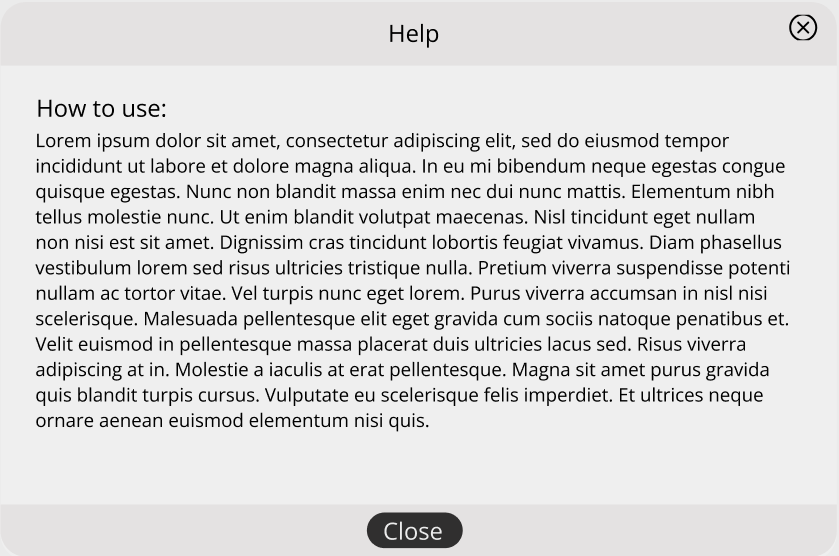
\includegraphics[width=\linewidth]{helpModal.png}
		\caption{User interface of the help modal/popup}
	\end{figure}
	
	\begin{figure}[H]
		\centering
		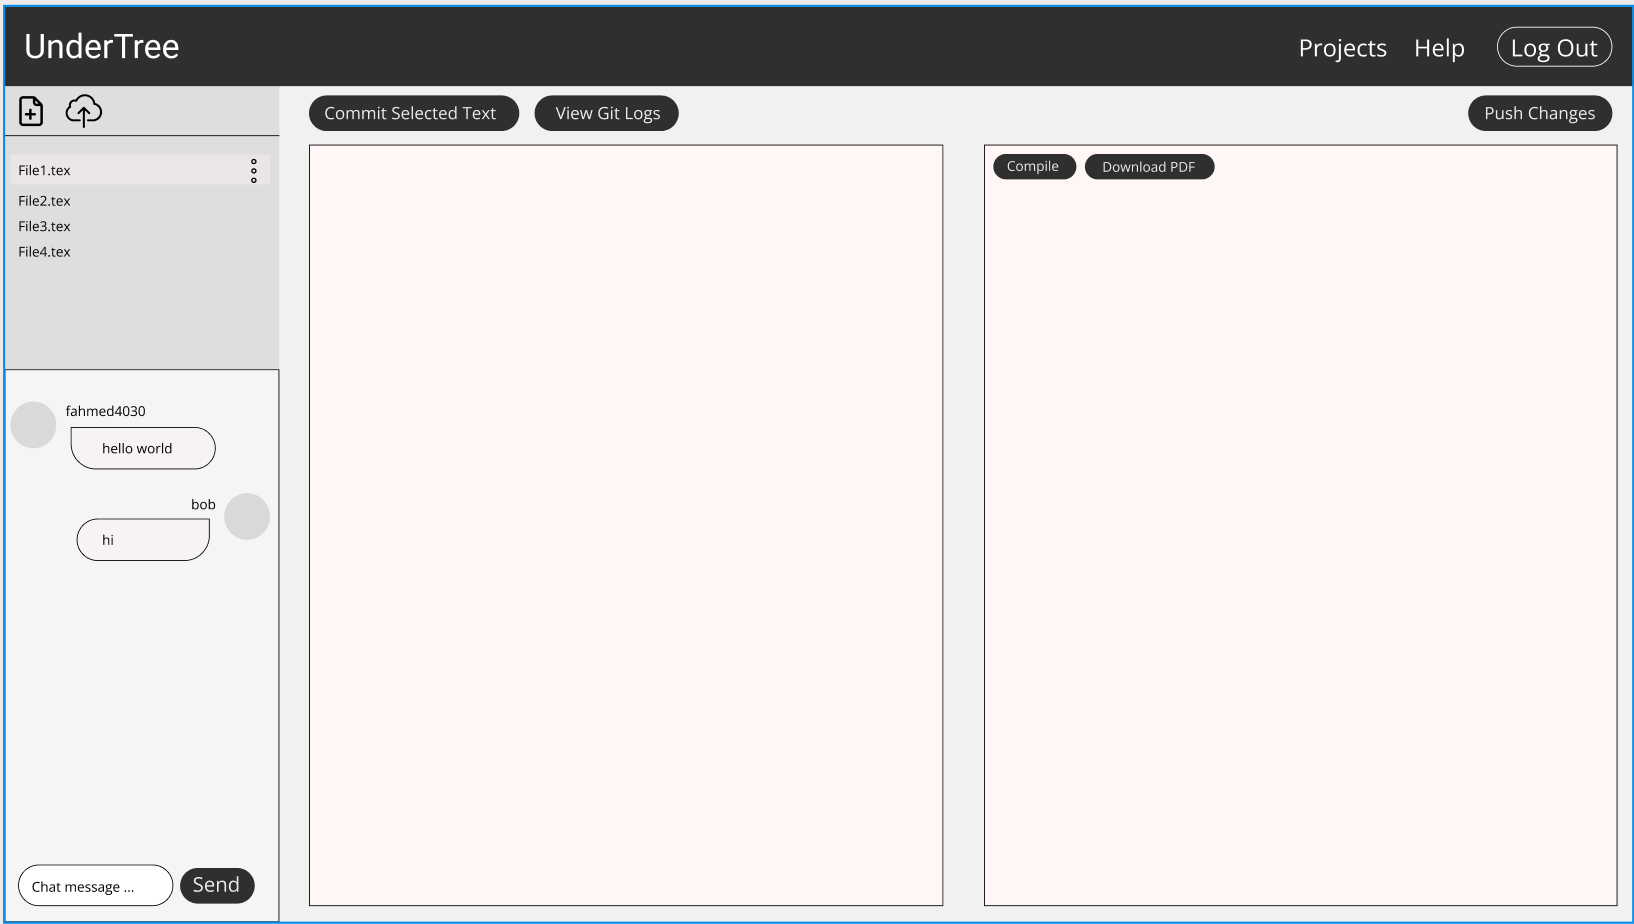
\includegraphics[width=\linewidth]{editorPage.png}
		\caption{User interface of the editor page}
	\end{figure}
	
	\begin{figure}[H]
		\centering
		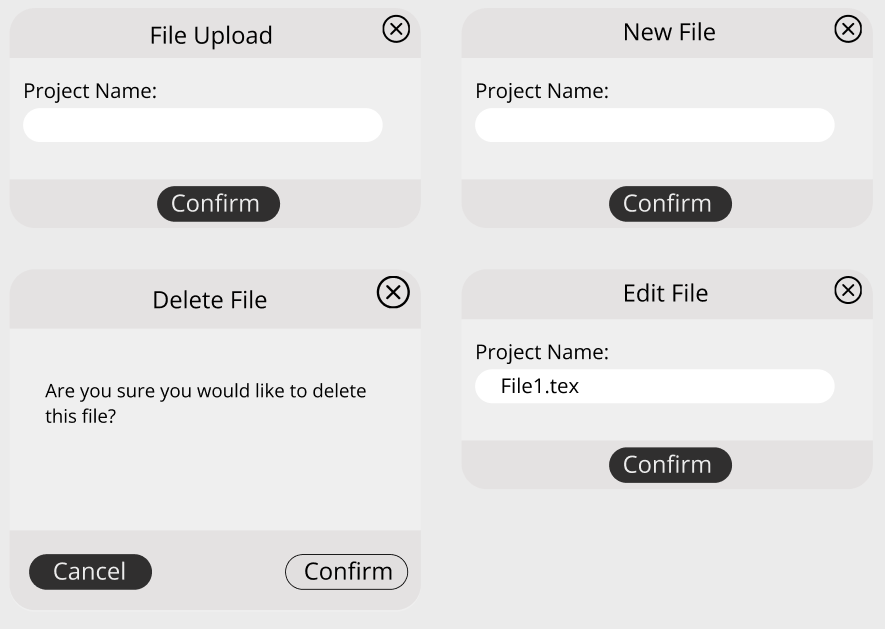
\includegraphics[width=\linewidth]{fileModals.png}
		\caption{User interface of the file related modals/popups}
	\end{figure}
	
	\begin{figure}[H]
		\centering
		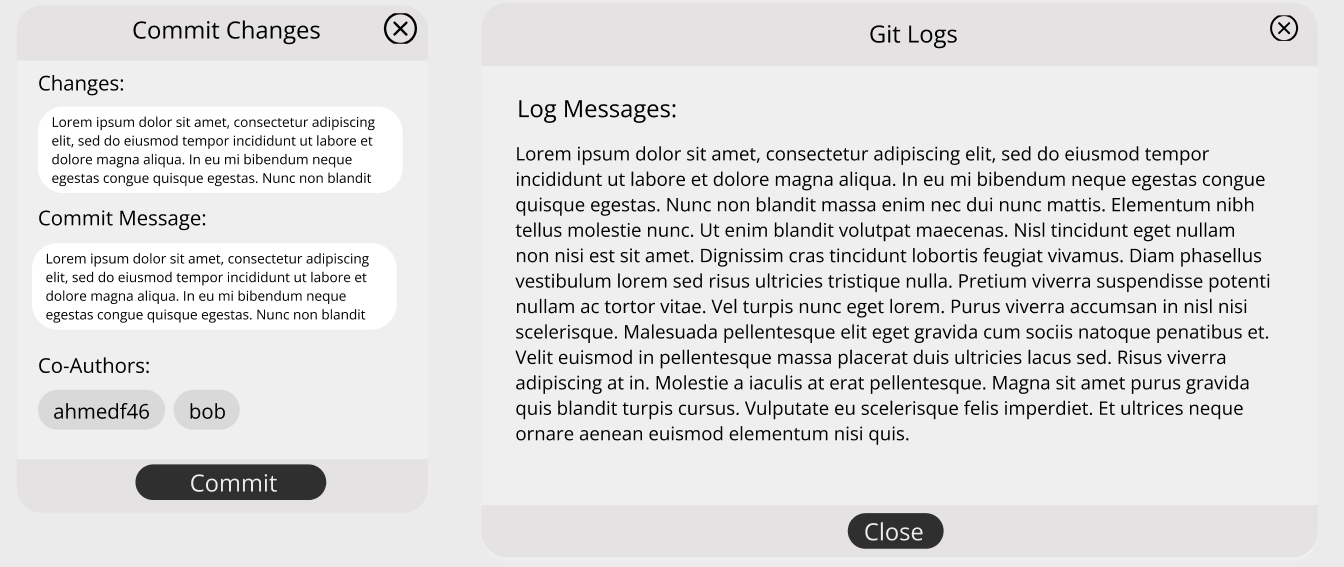
\includegraphics[width=\linewidth]{gitModals.png}
		\caption{User interface of the Git related modals/popups}
	\end{figure}
	
	\section{Design of Hardware}
	
	N/A
	
	\section{Design of Electrical Components}
	
	N/A
	
	\section{Design of Communication Protocols}
	
	The communication protocols used in this system are HTTP communication using an HTTP REST API server and a TCP socket that binds to connections on the HTTP server. Both these communication protocols are used to connect all elements of the UI to the back end services.
	
	\section{Timeline}
	
	
	% \wss{Schedule of tasks and who is responsible}
	\footnotesize\begin{longtable}{p{0.5\textwidth} p{0.3\textwidth}}
		\caption{Timeline based on module vs implementation plan}\\
		\toprule
		\textbf{Module} & \textbf{Implementation Plan}\\
		\midrule
		M1. Hardware-Hiding Module &  Already Implemented  \\
		M2. Project Editing Module &  Will be implemented by Veerash by January 25  \\
		M3. Editor Module &  Will be implemented by Veerash by February 10  \\
		M4. Syntax Highlighting Module &  Already Implemented  \\
		M5. Spelling Error Module &  Already Implemented  \\
		M6. File List Module &  Will be implemented by Veerash by January 31  \\
		M7. File Toolbar Module &  Will be implemented by Veerash by January 31  \\
		M8. New File Module &  Will be implemented by Veerash by January 25  \\
		M9. Upload File Module &  Will be implemented by Veerash by January 25  \\
		M10. User Cursors Module &  Already Implemented  \\
		M11. Text Highlighting Module &  Already Implemented  \\
		M12. File Synchronization Module &  Already Implemented  \\
		M13. File Services Module &  Will be implemented by Veerash by January 25  \\
		M14. File Database Interface Module &  Will be implemented by Veerash by January 25  \\
		M15. PDF Module &  Will be implemented by Faiq by February 10  \\
		M16. PDF Renderer Module &  Will be implemented by Faiq by February 1  \\
		M17. PDF Compiler Module &  Will be implemented by Faiq by February 1  \\
		M18. Chat Module &  Will be implemented by Faiq by February 10  \\
		M19. Chat Services Module &  Will be implemented by Faiq by February 11  \\
		M20. Chat Database Interface Module &  Will be implemented by Faiq by February 11  \\
		M21. Chat Socket Module &  Will be implemented by Faiq by February 11  \\
		M22. Chat Data Module &  Will be implemented by Faiq by February 11  \\
		M23. Instructions View Module &  Will be implemented by Faiq by February 11  \\
		M24. Projects Module &  Will be implemented by Eesha by February 11  \\
		M25. Project List Module &  Will be implemented by Eesha by February 10  \\
		M26. Project Deletion Module &  Will be implemented by Eesha by February 10  \\
		M27. Project Creation Module &  Will be implemented by Eesha by February 10  \\
		M28. New Project Module &  Will be implemented by Eesha by February 10  \\
		M29. Import Project Module  &  Will be implemented by Eesha by February 10 \\
		M30. Project Services Module &  Will be implemented by Eesha by February 10  \\
		M31. Project Database Interface Module &  Will be implemented by Eesha by February 10  \\
		M32. Project Data Module &  Will be implemented by Eesha by February 10  \\
		M33. GitHub Module &  Will be implemented by Kevin by February 10  \\
		M34. Auth Module &  Will be implemented by Kevin by February 10  \\
		M35. Login Controller Module &  Will be implemented by Kevin by February 10  \\
		M36. Logout Controller Module &  Will be implemented by Kevin by February 10  \\
		M37. Auth Service Module &  Will be implemented by Kevin by February 10  \\
		M38. Auth Database Interface Module &  Will be implemented by Kevin by February 10  \\
		M39. Auth Data Module &  Will be implemented by Kevin by February 10  \\
		M40. Navbar View Module &  Will be implemented by Kevin by February 10  \\
		M41. Check Permissions Module &  Will be implemented by Kevin by February 12  \\
		M42. Sync Module &  Will be implemented by Kevin by February 12  \\
		M43. Log Controller Module &  Will be implemented by Kevin by February 12  \\
		M44. Log View Module &  Will be implemented by Kevin by February 12  \\
		M45. Commit Controller Module &  Will be implemented by Kevin by February 5  \\
		M46. Commit View Module &  Will be implemented by Kevin by February 5  \\
		M47. Push Controller Module &  Will be implemented by Kevin by February 5  \\
		M48. Push View Module &  Will be implemented by Kevin by February 5  \\
		M51. MongoDB &  Already Implemented  \\
		Unit tests &  Will be created by March 8th by each team member responsible for the module  \\
		Revision 0 User Testing &  Will be carried out by the team by March 3rd \\
		Revision 1 User Testing &  Will be carried out by the team by March 31st \\
		\bottomrule
	\end{longtable}
	\normalsize
	% \bibliographystyle {plainnat}
	% \bibliography{../../../refs/References}
	
	\newpage{}
	
	\appendix
	
	\section{Interface}
	
	To help keep the user interface design responsive, we will be making use of the \href{https://getbootstrap.com/docs/4.1/getting-started/introduction/}{Bootstrap} CSS framework.
	
	\section{Mechanical Hardware}
	N/A
	
	\section{Electrical Components}
	N/A
	
	\section{Communication Protocols}
	
	We will be using pre-built services and libraries for these communication protocols, as a result a lot of information is not required on this topics. For HTTP communication, \href{https://caddyserver.com/docs/}{Caddy} will be used the server and REST API requests will be handled by \href{https://expressjs.com/en/guide/routing.html}{Express.js}. For TCP socket communication, we will be using the \href{https://socket.io/docs/v4/server-api/}{Socket.IO} library.
	
	\section{Reflection}
	
	The information in this section will be used to evaluate the team members on the
	graduate attribute of Problem Analysis and Design.  Please answer the following questions:
	
	\begin{enumerate}
		\item What are the limitations of your solution?  Put another way, given
		unlimited resources, what could you do to make the project better? (LO\_ProbSolutions)
		
		\begin{itemize}
			\item Veerash: A limitation of our solution is that there is some latency for doing real time synchronisation between the different users collaborating at the same time. This latency is heavily affected by network speeds and network latency, if we had infinite resources, we would not have to worry about this latency. But since that is not the case, we may have to use extra steps such as caching parts of the file that have not been edited to further reduce the latency.
			\item Faiq: A limitation of our solution is that running this service on a commercial server is extremely expensive due to the continuous communication aspect of it. To make the design simpler we could have used services such as lambda that are provided by AWS.
			\item Eesha: A current limitation of our solution is that it doesn't support a coding IDE. This would be a useful addition because it would provide users with a centralized application to both develop the code and then document it
			\item Kevin: The current limitation of the solution is that the system architecture could definitely be refactored and designed better to make things more optimized. 
			
		\end{itemize}
		
		
		\item Give a brief overview of other design solutions you considered.  What
		are the benefits and tradeoffs of those other designs compared with the chosen
		design?  From all the potential options, why did you select documented design?
		(LO\_Explores)
		
		\begin{itemize}
			\item Veerash: Other design solutions that was considered was using Broker Architecture for this application. But we quickly noticed the overhead that will be required the run the broker and the development effort to create the interfaces between the agents is not viable, thus we ended up going with a simple client server architecture. In the futre we may consider use Service Oriented Architecture to support the easy intergration of new feature into our application.
			\item Faiq: We considered designing the system using microservices, however this made the modules very thin and decreased the cohesion and increased the number of modules required for each module. A modified version of a model view controller fit our system better so that is what we ended up using.
			\item Eesha
			\item Kevin: The other design solution I considered was expanding the GitHub Services and Auth Services to separate modules for each type of service, the benefit of that would be the seperation of concerns. However this would add a lot more overhead and complications to design and implement.
			
		\end{itemize}
	\end{enumerate}
	
\end{document}